% Options for packages loaded elsewhere
\PassOptionsToPackage{unicode}{hyperref}
\PassOptionsToPackage{hyphens}{url}
%
\documentclass[
]{article}
\title{CSC8631 Report}
\author{Morgan Frodsham}
\date{03/12/2021}

\usepackage{amsmath,amssymb}
\usepackage{lmodern}
\usepackage{iftex}
\ifPDFTeX
  \usepackage[T1]{fontenc}
  \usepackage[utf8]{inputenc}
  \usepackage{textcomp} % provide euro and other symbols
\else % if luatex or xetex
  \usepackage{unicode-math}
  \defaultfontfeatures{Scale=MatchLowercase}
  \defaultfontfeatures[\rmfamily]{Ligatures=TeX,Scale=1}
\fi
% Use upquote if available, for straight quotes in verbatim environments
\IfFileExists{upquote.sty}{\usepackage{upquote}}{}
\IfFileExists{microtype.sty}{% use microtype if available
  \usepackage[]{microtype}
  \UseMicrotypeSet[protrusion]{basicmath} % disable protrusion for tt fonts
}{}
\makeatletter
\@ifundefined{KOMAClassName}{% if non-KOMA class
  \IfFileExists{parskip.sty}{%
    \usepackage{parskip}
  }{% else
    \setlength{\parindent}{0pt}
    \setlength{\parskip}{6pt plus 2pt minus 1pt}}
}{% if KOMA class
  \KOMAoptions{parskip=half}}
\makeatother
\usepackage{xcolor}
\IfFileExists{xurl.sty}{\usepackage{xurl}}{} % add URL line breaks if available
\IfFileExists{bookmark.sty}{\usepackage{bookmark}}{\usepackage{hyperref}}
\hypersetup{
  pdftitle={CSC8631 Report},
  pdfauthor={Morgan Frodsham},
  hidelinks,
  pdfcreator={LaTeX via pandoc}}
\urlstyle{same} % disable monospaced font for URLs
\usepackage[margin=1in]{geometry}
\usepackage{color}
\usepackage{fancyvrb}
\newcommand{\VerbBar}{|}
\newcommand{\VERB}{\Verb[commandchars=\\\{\}]}
\DefineVerbatimEnvironment{Highlighting}{Verbatim}{commandchars=\\\{\}}
% Add ',fontsize=\small' for more characters per line
\usepackage{framed}
\definecolor{shadecolor}{RGB}{248,248,248}
\newenvironment{Shaded}{\begin{snugshade}}{\end{snugshade}}
\newcommand{\AlertTok}[1]{\textcolor[rgb]{0.94,0.16,0.16}{#1}}
\newcommand{\AnnotationTok}[1]{\textcolor[rgb]{0.56,0.35,0.01}{\textbf{\textit{#1}}}}
\newcommand{\AttributeTok}[1]{\textcolor[rgb]{0.77,0.63,0.00}{#1}}
\newcommand{\BaseNTok}[1]{\textcolor[rgb]{0.00,0.00,0.81}{#1}}
\newcommand{\BuiltInTok}[1]{#1}
\newcommand{\CharTok}[1]{\textcolor[rgb]{0.31,0.60,0.02}{#1}}
\newcommand{\CommentTok}[1]{\textcolor[rgb]{0.56,0.35,0.01}{\textit{#1}}}
\newcommand{\CommentVarTok}[1]{\textcolor[rgb]{0.56,0.35,0.01}{\textbf{\textit{#1}}}}
\newcommand{\ConstantTok}[1]{\textcolor[rgb]{0.00,0.00,0.00}{#1}}
\newcommand{\ControlFlowTok}[1]{\textcolor[rgb]{0.13,0.29,0.53}{\textbf{#1}}}
\newcommand{\DataTypeTok}[1]{\textcolor[rgb]{0.13,0.29,0.53}{#1}}
\newcommand{\DecValTok}[1]{\textcolor[rgb]{0.00,0.00,0.81}{#1}}
\newcommand{\DocumentationTok}[1]{\textcolor[rgb]{0.56,0.35,0.01}{\textbf{\textit{#1}}}}
\newcommand{\ErrorTok}[1]{\textcolor[rgb]{0.64,0.00,0.00}{\textbf{#1}}}
\newcommand{\ExtensionTok}[1]{#1}
\newcommand{\FloatTok}[1]{\textcolor[rgb]{0.00,0.00,0.81}{#1}}
\newcommand{\FunctionTok}[1]{\textcolor[rgb]{0.00,0.00,0.00}{#1}}
\newcommand{\ImportTok}[1]{#1}
\newcommand{\InformationTok}[1]{\textcolor[rgb]{0.56,0.35,0.01}{\textbf{\textit{#1}}}}
\newcommand{\KeywordTok}[1]{\textcolor[rgb]{0.13,0.29,0.53}{\textbf{#1}}}
\newcommand{\NormalTok}[1]{#1}
\newcommand{\OperatorTok}[1]{\textcolor[rgb]{0.81,0.36,0.00}{\textbf{#1}}}
\newcommand{\OtherTok}[1]{\textcolor[rgb]{0.56,0.35,0.01}{#1}}
\newcommand{\PreprocessorTok}[1]{\textcolor[rgb]{0.56,0.35,0.01}{\textit{#1}}}
\newcommand{\RegionMarkerTok}[1]{#1}
\newcommand{\SpecialCharTok}[1]{\textcolor[rgb]{0.00,0.00,0.00}{#1}}
\newcommand{\SpecialStringTok}[1]{\textcolor[rgb]{0.31,0.60,0.02}{#1}}
\newcommand{\StringTok}[1]{\textcolor[rgb]{0.31,0.60,0.02}{#1}}
\newcommand{\VariableTok}[1]{\textcolor[rgb]{0.00,0.00,0.00}{#1}}
\newcommand{\VerbatimStringTok}[1]{\textcolor[rgb]{0.31,0.60,0.02}{#1}}
\newcommand{\WarningTok}[1]{\textcolor[rgb]{0.56,0.35,0.01}{\textbf{\textit{#1}}}}
\usepackage{graphicx}
\makeatletter
\def\maxwidth{\ifdim\Gin@nat@width>\linewidth\linewidth\else\Gin@nat@width\fi}
\def\maxheight{\ifdim\Gin@nat@height>\textheight\textheight\else\Gin@nat@height\fi}
\makeatother
% Scale images if necessary, so that they will not overflow the page
% margins by default, and it is still possible to overwrite the defaults
% using explicit options in \includegraphics[width, height, ...]{}
\setkeys{Gin}{width=\maxwidth,height=\maxheight,keepaspectratio}
% Set default figure placement to htbp
\makeatletter
\def\fps@figure{htbp}
\makeatother
\setlength{\emergencystretch}{3em} % prevent overfull lines
\providecommand{\tightlist}{%
  \setlength{\itemsep}{0pt}\setlength{\parskip}{0pt}}
\setcounter{secnumdepth}{-\maxdimen} % remove section numbering
\newlength{\cslhangindent}
\setlength{\cslhangindent}{1.5em}
\newlength{\csllabelwidth}
\setlength{\csllabelwidth}{3em}
\newlength{\cslentryspacingunit} % times entry-spacing
\setlength{\cslentryspacingunit}{\parskip}
\newenvironment{CSLReferences}[2] % #1 hanging-ident, #2 entry spacing
 {% don't indent paragraphs
  \setlength{\parindent}{0pt}
  % turn on hanging indent if param 1 is 1
  \ifodd #1
  \let\oldpar\par
  \def\par{\hangindent=\cslhangindent\oldpar}
  \fi
  % set entry spacing
  \setlength{\parskip}{#2\cslentryspacingunit}
 }%
 {}
\usepackage{calc}
\newcommand{\CSLBlock}[1]{#1\hfill\break}
\newcommand{\CSLLeftMargin}[1]{\parbox[t]{\csllabelwidth}{#1}}
\newcommand{\CSLRightInline}[1]{\parbox[t]{\linewidth - \csllabelwidth}{#1}\break}
\newcommand{\CSLIndent}[1]{\hspace{\cslhangindent}#1}
\ifLuaTeX
  \usepackage{selnolig}  % disable illegal ligatures
\fi

\begin{document}
\maketitle

\hypertarget{futurelearn-learning-analytics-for-newcastle-university}{%
\section{FutureLearn Learning Analytics for Newcastle
University}\label{futurelearn-learning-analytics-for-newcastle-university}}

\hypertarget{business-understanding}{%
\subsection{Business understanding}\label{business-understanding}}

\hypertarget{background}{%
\subsubsection{Background}\label{background}}

This report details the process and findings of exploratory data
analysis for Newcastle University's FutureLearn course called ``Cyber
Security: Safety at Home, Online, in Life.'' Data analysis of
educational platforms, such as FutureLearn, is a key part of learning
analytics, which is defined as \emph{``the measurement, collection,
analysis and reporting of data about learners and their contexts, for
purposes of understanding and optimising learning and the environments
in which it occurs.''}
(\protect\hyperlink{ref-Learning-Analytics-Conference}{\emph{1st
International Conference on Learning Analytics and Knowledge}}
(\protect\hyperlink{ref-Learning-Analytics-Conference}{2011})) Learning
analytics has the potential to help educational institutions undertake
data-driven decision-making (\protect\hyperlink{ref-EDUCAUSE}{Long and
Siemens} (\protect\hyperlink{ref-EDUCAUSE}{2011})) that better support
learners through their learning journey
(\protect\hyperlink{ref-Bricks}{Shacklock}
(\protect\hyperlink{ref-Bricks}{2016})).

\hypertarget{business-objectives-and-success-criteria}{%
\subsubsection{Business objectives and success
criteria}\label{business-objectives-and-success-criteria}}

FutureLearn is a massive open online course (MOOC) provider. It promotes
itself as \emph{``a powerful new way to learn online''}
(\protect\hyperlink{ref-FutureLearn}{FutureLearn}
(\protect\hyperlink{ref-FutureLearn}{n.d.})), designed with the
principles of effective learning in mind. A core objective of
FutureLearn is, therefore, to improve learning effectiveness. Learning
effectiveness can be indicated by learner engagement, their success
rate, and completion time (\protect\hyperlink{ref-E-learning}{S.
Hubalovsky and Musilek} (\protect\hyperlink{ref-E-learning}{2018})).

The objective of the exploratory data analysis outlined by this report
is to better understand the learning effectiveness of Newcastle
University's Future Learn Cyber Security course. The process and
findings described by this report explore the question: ``Do learners
have a higher chance of success the more data they share with
FutureLearn?'' Here, ``a higher chance of success'' is that learners are
more likely to complete the course. The data shared by learners refers
to the optional data requested by FutureLearn; specifically, the
provision of personal identifiers like demographic information
(demographic data will be used as the short hand for this). In this
project, the provision of this data is taken to be an indicator of
learner engagement. For this analysis the business success criteria is
to give useful insights into the relationship between learners'
demographic data (as a proxy for learner engagement) and learner success
rate.

Other business objectives that were considered included:

\begin{itemize}
\item
  Do learners who complete the course, complete it more quickly?
\item
  From which countries are learners more likely to engage with the
  course?
\item
  Do learners have a higher chance of success the more times they
  interact with the future learn platform?
\end{itemize}

These objectives have not been pursued by this project because they are
concerned with later stages of the learners' journey through the course.
Instead, this project focused on the impact of learners initial
engagement with FutureLearn (by providing demographic data when they
enrol) on their completion of the course, and therefore their ultimate
success.

\hypertarget{costs-and-benefits}{%
\subsubsection{Costs and benefits}\label{costs-and-benefits}}

This is a low cost, light resource project (as outlined by the resource
inventory below). If the analysis and findings outlined by this report
are significant, there could be business benefits. For example, the
analysis findings could help Newcastle University and FutureLearn
support learners to succeed, increasing learner satisfaction and, if
desired, could lead to increase of learners for both organisations.

\hypertarget{project-plan}{%
\subsubsection{Project plan}\label{project-plan}}

Started on 8 November 2021, the deadline for this project is 16:30, 3
December 2021. The first iteration, between 8 and 18 November, focused
on project set up, understanding what data was provided, learning R and
practicing with the technical suite. The second and third iteration are
highly dependent on the success of the first iteration. The second
iteration, between 19 and 25 November, focused on tidying the data,
exploring potential routes of analysis and setting up the
ProjectTemplate configurations for this project. The third iteration,
between 29 November and 3 December focused on deeper exploratory data
analysis and creating project outputs, such as the report and graphs
desired.

The resources required for this project, as well as inputs (resources,
tools and techniques) and outputs, are outlined in other sections of
this report.

\hypertarget{terminology}{%
\subsubsection{Terminology}\label{terminology}}

The terminology used throughout this report includes:

\begin{itemize}
\item
  R, which is a programming language for statistical computing and
  graphics.
\item
  RStudio, which is an Interated Development Environment for R.
\item
  R packages, which are extensions to the R statistcial programming
  language. R packages contain code, data, and documentation in a
  standardised collection format that can be installed by users of R.
  The R packages used by this report are listed in the section below.
\item
  Git, which is software for tracking changes in any set of files,
  usually used for coordinating work among programmers collaboratively
  developing source code. GitHub is a provider of internet hosting for
  software development and version control using Git. Git Bash is an
  application for Microsoft Windows environments which provides an
  emulation layer for a Git command line experience.
\item
  Tibble, which is a data frame that stores data in R and appears as a
  table.
\item
  Success rate, which is the number of learners who have completed the
  course divided by the total number of learners as a percentage.
\end{itemize}

\hypertarget{inventory-of-resources}{%
\subsubsection{Inventory of resources}\label{inventory-of-resources}}

This project has been undertaken by one part-time person, on a Dell G7
17'' laptop. Git, RStudio and a selection of R packages (detailed in the
next section) have been used to deliver the project. Newcastle
University also provided data from its FutureLearn cyber security course
for analysis.

\hypertarget{initial-assessment-of-tools-and-techniques}{%
\subsubsection{Initial assessment of tools and
techniques}\label{initial-assessment-of-tools-and-techniques}}

This project utilises the following tools and techniques:

\begin{itemize}
\item
  CRISP-DM (\protect\hyperlink{ref-CRISP-DM}{Chapman et. al. and Wirth}
  (\protect\hyperlink{ref-CRISP-DM}{2000})) is the methodology used to
  deliver data workflow best practice;
\item
  Tidyverse for R is the R package used for the analysis;
\item
  ggplot2 for R is the R package used for visualisations;
\item
  RColorBrewer is the R package used to provide accessible colour
  palettes for visualisations;
\item
  ProjectTemplate is the R package used to improve the reproducibility
  of this analysis;
\item
  Git (specifically GitHub and GitBash) is used for version control;
\item
  all written documentation is created with the R package, RMarkdown;
  and
\item
  natbib is an R package used for the bibliography.
\end{itemize}

\hypertarget{requirements-assumptions-and-constraints}{%
\subsubsection{Requirements, assumptions and
constraints}\label{requirements-assumptions-and-constraints}}

This project, as well as the process and findings outlined in this
report, is limited to the data analysis pipeline. Consequently, there is
no modelling or deployment section in this report either. The type of
project results to be expected are initial findings from exploratory
analysis, graphical summaries of these findings and explanatory text.

To conduct the analysis outlined by this report, it is assumed that the
data is accurate. Where there is a missing value (often represented as
NA), it is assumed that this data value does not apply to the learner or
the learner did not provide FutureLearn with that type of data. It is
assumed that the data vales of fully\_participated\_at (inside the
enrolments data set) demonstrate whether learners have completed the
course or not. If this assumption is incorrect, it will have a
significant impact on the project findings. It is also assumed that it
is optional for the learners to complete the demographic data (inside
the enrolments data set, like gender or country, or the archetype data
set) as there is a high number of missing values. If this assumption is
incorrect, the data should not be interpreted as a proxy of learner
engagement.

\hypertarget{risks-and-contingencies}{%
\subsubsection{Risks and contingencies}\label{risks-and-contingencies}}

Due to the limited nature of this project, there is a strong risk that
there are confounding variables, which could cause a spurious
association. More comprehensive analysis of all the data sets would be
required to determine this and provde the correlations uncovered in the
analysis findings. Therefore, all findings outlined by this report are
to be interpreted with caution.

Similarly, the assumptions outlined in the section above pose a risk to
this project. Regular communication with key Newcastle University staff
members has helped to mitigate this risk. However, it should be noted
that FutureLearn has not been contacted for this report. This will be
vital to mitigating the risk if further analysis and modelling is
undertaken beyond this project.

This project has also attempted to address common programming risks such
as unrepeatable code and opaque decision-making by using ProjectTemplate
and Git for current best practice in programming transparency and
reproducibility.

\hypertarget{data-mining-goals-and-success-criteria}{%
\subsubsection{Data mining goals and success
criteria}\label{data-mining-goals-and-success-criteria}}

The exploratory data analysis outlined by this report explores the
question: ``Do learners have a higher chance of success the more data
they share with FutureLearn?'' To understand this, the data mining aims
to determine:

\begin{enumerate}
\def\labelenumi{\arabic{enumi}.}
\item
  What is the gross success rate of learners? The data mining success
  criteria is the percentage of all learners who complete the course.
\item
  How many learners provide any demographic data? The data mining
  success criteria is the percentage of all learners who provide
  optional demographic data such as gender, age range or employment
  status from the enrolments data set.
\item
  What is the success rate of learners who provide demographic data? The
  data mining success criteria is the percentage of learners who
  complete the course and provide demographic data (as outlined in point
  2).
\item
  What is the success rate of learners who do not provide demographic
  data? The data mining success criteria is the percentage of learners
  who complete the course and do not provide any demographic data (as
  outlined in point 2).
\item
  Is there any correlation between learners' success and the provision
  of demographic data? The data mining success criteria is the
  difference between the success rates od learners who provided or did
  not provide demographic data (using the findings from point 3 and 4).
\end{enumerate}

\hypertarget{data-understanding}{%
\subsection{Data understanding}\label{data-understanding}}

\hypertarget{initial-data-collection}{%
\subsubsection{Initial data collection}\label{initial-data-collection}}

Newcastle University's FutureLearn cyber security course has run seven
times. The first run provided six different data sets, the second run
provided seven, and the others provided eight. There are 53 different
data sets for potential exploration. In total, 53 data sets have been
provided by Newcastle University.

It is unclear whether there have been any problems in data acquisition
or extraction as Newcastle University has provided the data.

\hypertarget{data-description}{%
\subsubsection{Data description}\label{data-description}}

The first run of Newcastle University's FutureLearn cyber security
course provides the following data sets:

\begin{itemize}
\item
  archetype survey responses (id, learner\_id, responded\_at,
  archetype);
\item
  enrolments (learner\_id, enrolled\_at, unenrolled\_at role,
  fully\_participated\_at, purchased\_statement\_at gender, country
  age\_range, highest\_education\_level, employment\_status,
  employment\_area detected\_country);
\item
  leaving survey responses (id, learner\_id, left\_at leaving\_reason,
  last\_completed\_step\_at, last\_completed\_step,
  last\_completed\_week\_number, last\_completed\_step\_number);
\item
  question responses (learner\_id, quiz\_question, question\_type,
  week\_number, step\_number, question\_number, response,
  cloze\_response, submitted\_at, correct);
\item
  step activity (learner\_id step, week\_number step\_number,
  first\_visited\_at, last\_completed\_at); and
\item
  weekly sentiment survey (id responded\_at, week\_number,
  experience\_rating, reason).
\end{itemize}

The second run provides the same data sets as well as a data sets
specifying:

\begin{itemize}
\tightlist
\item
  team members (id, first\_name, last\_name, team\_role, user\_role).
\end{itemize}

The other five runs provide the same data sets as the second run as well
as a data set on:

\begin{itemize}
\tightlist
\item
  video stats (step\_position, title video\_duration, total\_views,
  total\_downloads, total\_caption\_views, total\_transcript\_views,
  viewed\_hd, viewed\_five\_percent, viewed\_ten\_percent,
  viewed\_twentyfive\_percent, viewed\_fifty\_percent,
  viewed\_seventyfive\_percent, viewed\_ninetyfive\_percent,
  viewed\_onehundred\_percent, console\_device\_percentage,
  desktop\_device\_percentage, mobile\_device\_percentage,
  tv\_device\_percentage, tablet\_device\_percentage,
  unknown\_device\_percentage, europe\_views\_percentage,
  oceania\_views\_percentage, asia\_views\_percentage,
  north\_america\_views\_percentage, south\_america\_views\_percentage,
  africa\_views\_percentage, antarctica\_views\_percentage).
\end{itemize}

\hypertarget{data-quality}{%
\subsubsection{Data quality}\label{data-quality}}

The data provided by Newcastle University is raw, and so its accuracy is
assumed. The completeness of the data varies by the run of the course;
for example, the data collected by the first run of the course is
relatively sparse compared to the seventh run of the course. In runs
three and four more data is being collected; this could be because there
are fewer optional sections (such as the archetype or leaving survey),
but it is unknown why this change has occurred. There are also missing
values in data sets where learners have not completed the course (or
particular parts of it) and when learners have not provided optional
data (as outlined above).

\hypertarget{data-exploration}{%
\subsubsection{Data exploration}\label{data-exploration}}

To address the business objective and success criteria, the exploratory
analysis outlined by this report uses the enrolments data set because it
includes the field fully\_participated\_at, which is considered to mean
course completion, as well as learners' demographic data. This section
is structured by the data mining goals.

\textbf{Goal 1 (Gross Success Rate)}

To understand the success rate of all learners who undertake the course,
the total number of learners who have undertaken the course across all
seven runs needs to be determined. All seven runs were combined, two
filters were created to show how many learners completed (complete) and
did not complete the course (incomplete).

\begin{Shaded}
\begin{Highlighting}[]
\CommentTok{\# Identify how many learners there are in all seven runs.}
\NormalTok{total\_learners }\OtherTok{\textless{}{-}}\NormalTok{ (}\DecValTok{2154}\SpecialCharTok{+}\DecValTok{35142}\NormalTok{) }\SpecialCharTok{\%\textgreater{}\%} \CommentTok{\# Adding complete and incomplete totals.}
  \FunctionTok{print}\NormalTok{()}
\end{Highlighting}
\end{Shaded}

\begin{verbatim}
## [1] 37296
\end{verbatim}

\begin{Shaded}
\begin{Highlighting}[]
\CommentTok{\# Calculate the success rate of all learners who enrolled in the course. }
\NormalTok{SR\_gross }\OtherTok{\textless{}{-}}\NormalTok{ (}\DecValTok{100}\SpecialCharTok{*}\NormalTok{(}\DecValTok{2154}\SpecialCharTok{/}\NormalTok{total\_learners)) }\SpecialCharTok{\%\textgreater{}\%} 
  \FunctionTok{round}\NormalTok{(., }\AttributeTok{digits =} \DecValTok{2}\NormalTok{) }\SpecialCharTok{\%\textgreater{}\%} 
  \FunctionTok{print}\NormalTok{()}
\end{Highlighting}
\end{Shaded}

\begin{verbatim}
## [1] 5.78
\end{verbatim}

This allows us to determine that there are 37,296 learners who have
enrolled in Newcastle University's FutureLearn cyber security course,
and 5.78\% of them have completed it, which is the gross success rate.

\textbf{Goal 2 (Demographic Data)}

For the enrolments data set, demographic data refers to the following
fields that learners could provide:

\begin{itemize}
\item
  gender,
\item
  country,
\item
  age\_range,
\item
  highest\_education\_level,
\item
  employment\_status, and
\item
  employment\_area.
\end{itemize}

To investigate whether learners had provided any of this demographic
data, a data set called `FL1' was created with new columns (that
corresponded to the aforementioned demographic data) showing TRUE or
FALSE for whether the learner had shared that type of demographic data.

\begin{Shaded}
\begin{Highlighting}[]
\CommentTok{\# Create a new column called "count" in FL1 containing the value (count of }
\CommentTok{\# columns) where there is a a vale != FALSE.}
\NormalTok{true\_counts }\OtherTok{\textless{}{-}}\NormalTok{ FL1 }\SpecialCharTok{\%\textgreater{}\%} 
  \FunctionTok{mutate}\NormalTok{(}\AttributeTok{num\_true =} \FunctionTok{rowSums}\NormalTok{(.[ids\_of\_declared\_cols] }\SpecialCharTok{!=} \ConstantTok{FALSE}\NormalTok{)) }\CommentTok{\# Count up how }
\CommentTok{\# many of the columns have a value != FALSE.}

\CommentTok{\# Count the number of demographic columns filled in by the learner who completed}
\CommentTok{\# and did not complete the course.}
\NormalTok{learner\_counts }\OtherTok{\textless{}{-}}\NormalTok{ true\_counts }\SpecialCharTok{\%\textgreater{}\%} 
  \FunctionTok{group\_by}\NormalTok{(num\_true, completed) }\SpecialCharTok{\%\textgreater{}\%} 
  \FunctionTok{count}\NormalTok{()}

\CommentTok{\# Display a tibble of learners who have completed or not completed the course, }
\CommentTok{\# counting number of demographic columns filled in by the learner. }
\NormalTok{learner\_counts }\SpecialCharTok{\%\textgreater{}\%}
  \FunctionTok{print}\NormalTok{(ids\_of\_declared\_cols, true\_counts, }\AttributeTok{n =} \DecValTok{15}\NormalTok{, }\AttributeTok{width =} \ConstantTok{Inf}\NormalTok{)}
\end{Highlighting}
\end{Shaded}

\begin{verbatim}
## # A tibble: 15 x 3
## # Groups:   num_true, completed [15]
##    num_true completed     n
##       <dbl> <lgl>     <int>
##  1        0 FALSE     31467
##  2        0 TRUE       1626
##  3        1 FALSE        14
##  4        2 FALSE        15
##  5        2 TRUE          4
##  6        3 FALSE        31
##  7        3 TRUE          9
##  8        4 FALSE        79
##  9        4 TRUE          7
## 10        5 FALSE       858
## 11        5 TRUE        134
## 12        6 FALSE      2676
## 13        6 TRUE        372
## 14       NA FALSE         2
## 15       NA TRUE          2
\end{verbatim}

This table shows us how many learners who have completed (TRUE) or not
completed (FALSE) the course have provided demographic data and, if so,
how many demographic data fields they have provided.

There are four instances of NA in the table that should be investigated
further; for now, it is assumed that these learners did not provide
demographic data.

Below shows that 4,199 learners provided demographic data.

\begin{Shaded}
\begin{Highlighting}[]
\CommentTok{\# Calculate the number of learners who provided demographic data}
\NormalTok{d\_count }\OtherTok{\textless{}{-}}\NormalTok{ (}\DecValTok{37296} \SpecialCharTok{{-}} \DecValTok{31467} \SpecialCharTok{{-}} \DecValTok{1626} \SpecialCharTok{{-}} \DecValTok{4}\NormalTok{) }\SpecialCharTok{\%\textgreater{}\%}
  \FunctionTok{print}\NormalTok{()}
\end{Highlighting}
\end{Shaded}

\begin{verbatim}
## [1] 4199
\end{verbatim}

\textbf{Goal 3 (Demographic Data Success Rate)}

The table in Goal 2 shows us how many learners provided demographic data
and completed the course. This enables us to calculate the success rate
of learners who have provided demographic data.

\begin{Shaded}
\begin{Highlighting}[]
\CommentTok{\# Calculate how many learners provided demographic data.}
\NormalTok{d\_complete\_count }\OtherTok{\textless{}{-}}\NormalTok{ (}\DecValTok{4}\SpecialCharTok{+}\DecValTok{9}\SpecialCharTok{+}\DecValTok{7}\SpecialCharTok{+}\DecValTok{134}\SpecialCharTok{+}\DecValTok{372}\NormalTok{) }\SpecialCharTok{\%\textgreater{}\%}
  \FunctionTok{print}\NormalTok{ ()}
\end{Highlighting}
\end{Shaded}

\begin{verbatim}
## [1] 526
\end{verbatim}

\begin{Shaded}
\begin{Highlighting}[]
\CommentTok{\# Calculate the success rate of learners who provided demographic data.}
\NormalTok{SR\_d }\OtherTok{\textless{}{-}}\NormalTok{ (}\DecValTok{100}\SpecialCharTok{*}\NormalTok{(}\FunctionTok{as.numeric}\NormalTok{(d\_complete\_count))}\SpecialCharTok{/}\NormalTok{(}\FunctionTok{as.numeric}\NormalTok{(d\_count))) }\SpecialCharTok{\%\textgreater{}\%}
  \FunctionTok{round}\NormalTok{(., }\AttributeTok{digits =} \DecValTok{2}\NormalTok{) }\SpecialCharTok{\%\textgreater{}\%}
  \FunctionTok{print}\NormalTok{()}
\end{Highlighting}
\end{Shaded}

\begin{verbatim}
## [1] 12.53
\end{verbatim}

This allows us to determine that of the 4,199 learners who provided
demographic data, 526 completed the course. The success rate of learners
who provide demographic data is 12.53\%.

\textbf{Goal 4 (No Demographic Data Success Rate)}

The table created as part of Goal 2 shows how many learners did not
complete the course and did not provide demographic data.

\begin{Shaded}
\begin{Highlighting}[]
\CommentTok{\# Calculate how many learners did not provide demographic data.}
\NormalTok{no\_d\_count }\OtherTok{\textless{}{-}}\NormalTok{ (}\DecValTok{31467}\SpecialCharTok{+}\DecValTok{1626}\SpecialCharTok{+}\DecValTok{2}\SpecialCharTok{+}\DecValTok{2}\NormalTok{) }\SpecialCharTok{\%\textgreater{}\%}
  \FunctionTok{print}\NormalTok{()}
\end{Highlighting}
\end{Shaded}

\begin{verbatim}
## [1] 33097
\end{verbatim}

\begin{Shaded}
\begin{Highlighting}[]
\CommentTok{\# Calculate how many of those learners completed the course.}
\NormalTok{no\_d\_complete\_count }\OtherTok{\textless{}{-}}\NormalTok{ (}\DecValTok{1626}\SpecialCharTok{+}\DecValTok{2}\NormalTok{) }\SpecialCharTok{\%\textgreater{}\%}
  \FunctionTok{print}\NormalTok{()}
\end{Highlighting}
\end{Shaded}

\begin{verbatim}
## [1] 1628
\end{verbatim}

\begin{Shaded}
\begin{Highlighting}[]
\CommentTok{\# Calculate success rate of learners who did not provide demographic data.}
\NormalTok{SR\_no\_d }\OtherTok{\textless{}{-}}\NormalTok{ (}\DecValTok{100}\SpecialCharTok{*}\NormalTok{(}\FunctionTok{as.numeric}\NormalTok{(no\_d\_complete\_count))}\SpecialCharTok{/}\NormalTok{(}\FunctionTok{as.numeric}\NormalTok{(no\_d\_count))) }\SpecialCharTok{\%\textgreater{}\%}
  \FunctionTok{round}\NormalTok{(., }\AttributeTok{digits =} \DecValTok{2}\NormalTok{) }\SpecialCharTok{\%\textgreater{}\%}
  \FunctionTok{print}\NormalTok{()}
\end{Highlighting}
\end{Shaded}

\begin{verbatim}
## [1] 4.92
\end{verbatim}

This allows us to determine that of the 33,097 learners who did not
provide demographic data, 1,628 learners did not complete the course.
The success rate of learners who do not provide demographic data is
4.92\%.

\textbf{Goal 5 (Potential Correlation)}

We have identified three different success rates for learners:

\begin{verbatim}
## # A tibble: 3 x 2
##   Success_Rate        Percentage
##   <chr>                    <dbl>
## 1 Gross                     5.78
## 2 No Demographic Data       4.92
## 3 Demographic Data         12.5
\end{verbatim}

It appears there may be a correlation between learners' success rate and
their provision of demographic data (as a proxy for learner engagement);
learners who provide demographic data are over twice as likely (2.55x)
to complete the course than learners who do not provide demographic
data.

\hypertarget{business-understanding-second-iteration}{%
\subsection{Business understanding (second
iteration)}\label{business-understanding-second-iteration}}

\hypertarget{business-objectives-and-success-criteria-1}{%
\subsubsection{Business objectives and success
criteria}\label{business-objectives-and-success-criteria-1}}

Our core objective is to determine whether learners have a higher chance
of success the more data they share with FutureLearn. An initial
investigation into the data provided by Newcastle University suggests
that learners do have a higher chance of success the more data they
share with FutureLearn. However, the business success criteria is to
give useful insights into the relationship between learner engagement
and learner success rate. A better understanding of the correlation
between learners' success rate and their provision of demographic data
is therefore needed.

\hypertarget{data-mining-goals-and-success-criteria-1}{%
\subsubsection{Data mining goals and success
criteria}\label{data-mining-goals-and-success-criteria-1}}

To better understand the relationship between learners' engagement and
success rate. The gender, age, level of education and employment status
of learners have been chosen as the demographic data fields for further
exploration as there are fewer categories in each field by comparison to
country and employment status. The second iteration of data mining aims
to determine:

2.1. Which genders declared by learners have a higher chance of success?
The data mining success criteria is the percentage of learners who have
completed the course for each gender declared.

2.2. Which ages declared by learners have a higher chance of success?
The data mining success criteria is the percentage of learners who have
completed the course for each age range declared.

2.3. Which levels of education declared by the learners have a higher
chance of success? The data mining success criteria is the percentage of
learners who have completed the course for each age range declared.

2.4. Which employment statuses declared by learners have a higher chance
of success? The data mining success criteria is the percentage of
learners who have completed the course for each employment status
declared.

\hypertarget{data-understanding-second-iteration}{%
\subsection{Data understanding (second
iteration)}\label{data-understanding-second-iteration}}

The details of data collection, description and quality outlined in the
first iteration of data understanding also apply to this second
iteration.

\hypertarget{data-exploration-1}{%
\subsubsection{Data exploration}\label{data-exploration-1}}

This second iteration of data exploration also uses the enrolments data
set, with the same caveats as the first iteration. This section is also
structured by the data mining goals.

\textbf{Goal 2.1 (Gender Success Rate)}

Using true\_counts from Goal 2 in the first iteration of data
exploration we can determine that 4159 learners declared their gender to
FutureLearn.

\begin{Shaded}
\begin{Highlighting}[]
\CommentTok{\# Identify which genders completed or did not complete the course.}
\NormalTok{gender\_counts }\OtherTok{\textless{}{-}}\NormalTok{ true\_counts }\SpecialCharTok{\%\textgreater{}\%}
  \FunctionTok{group\_by}\NormalTok{(num\_true, gender, completed) }\SpecialCharTok{\%\textgreater{}\%}
  \FunctionTok{count}\NormalTok{() }\SpecialCharTok{\%\textgreater{}\%}
  \FunctionTok{filter}\NormalTok{(}\SpecialCharTok{!}\NormalTok{(gender }\SpecialCharTok{==} \StringTok{"Unknown"}\NormalTok{))}

\CommentTok{\# Total learners who declared their gender.}
\NormalTok{total\_gender }\OtherTok{\textless{}{-}} \FunctionTok{sum}\NormalTok{(gender\_counts}\SpecialCharTok{$}\NormalTok{n) }\SpecialCharTok{\%\textgreater{}\%} 
  \FunctionTok{print}\NormalTok{()}
\end{Highlighting}
\end{Shaded}

\begin{verbatim}
## [1] 4159
\end{verbatim}

\begin{Shaded}
\begin{Highlighting}[]
\CommentTok{\# Total learners who declared their gender and completed the course.}
\NormalTok{c\_total\_gender }\OtherTok{\textless{}{-}}\NormalTok{ (}\DecValTok{3} \SpecialCharTok{+} \DecValTok{1} \SpecialCharTok{+} \DecValTok{1} \SpecialCharTok{+} \DecValTok{4} \SpecialCharTok{+} \DecValTok{6} \SpecialCharTok{+} \DecValTok{60} \SpecialCharTok{+} \DecValTok{60} \SpecialCharTok{+} \DecValTok{1} \SpecialCharTok{+} \DecValTok{132} \SpecialCharTok{+} \DecValTok{239} \SpecialCharTok{+} \DecValTok{1} \SpecialCharTok{+} \DecValTok{2}\NormalTok{ )}

\CommentTok{\# Calculate success rate of those who provided their gender.}
\NormalTok{SR\_total\_gender }\OtherTok{\textless{}{-}}\NormalTok{ (}\DecValTok{100}\SpecialCharTok{*}\NormalTok{(c\_total\_gender}\SpecialCharTok{/}\NormalTok{total\_gender)) }\SpecialCharTok{\%\textgreater{}\%}
  \FunctionTok{round}\NormalTok{(., }\AttributeTok{digits =} \DecValTok{2}\NormalTok{) }\SpecialCharTok{\%\textgreater{}\%}
  \FunctionTok{print}\NormalTok{()}
\end{Highlighting}
\end{Shaded}

\begin{verbatim}
## [1] 12.26
\end{verbatim}

This allows us to determine that the success rate of learners who
declare their gender is 12.26\%. The graph below was created to
understand whether the success rate varies for different genders
declared by learners.

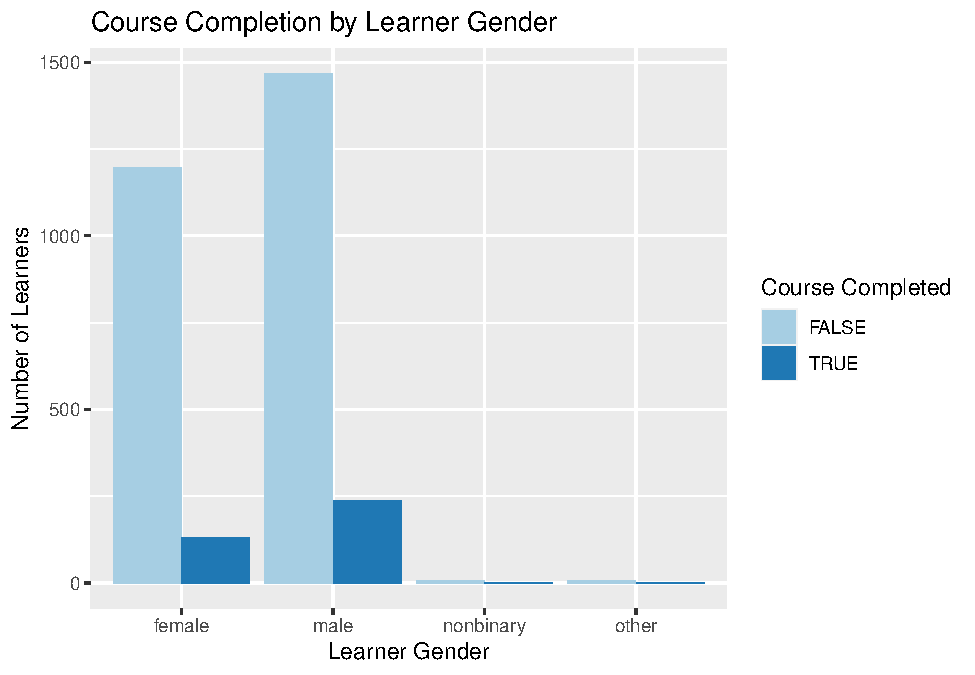
\includegraphics{CSC8631-Report---210431461_files/figure-latex/gender_completion-1.pdf}
This graph indicates that those who identify as male may be more likely
to complete the course. This is unclear, however, because there seems to
be a proportionate number of learners who identify as male, but do not
complete the course.

To better understand the results of this graph, the table below was
created. The table was created through the same process used to create
the gender success rate (as above) by applying it to each declared
gender (the code can be found in the file \texttt{eda2.R} located in the
\texttt{src} folder).

\begin{verbatim}
## # A tibble: 5 x 2
##   Success_Rate Percentage
##   <chr>             <dbl>
## 1 Gender            12.3 
## 2 Male              14.0 
## 3 Female            10.7 
## 4 Nonbinary          8.33
## 5 Other              7.14
\end{verbatim}

The table shows us that of learners who declared their gender, those who
identified as male had a higher chance of success (14.02\%) than people
who identified as another gender. Those who identified as other had the
lowest chance of success (7.14\%).

The graph below was created to better understand the provision of
demographic data by learners who declared their gender.

\begin{verbatim}
## Warning: Removed 3 rows containing missing values (geom_bar).
\end{verbatim}

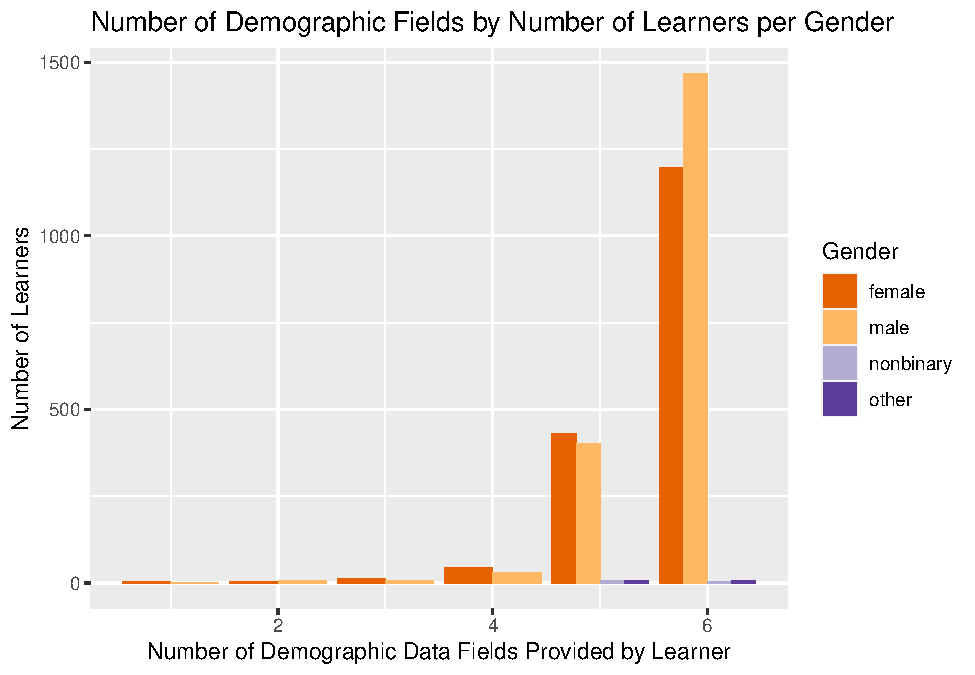
\includegraphics{CSC8631-Report---210431461_files/figure-latex/gender_demographic_declared-1.pdf}

This graph indicates that learners who identify as male are more likely
to declare all six demographic data values than women. Similarly, if a
learner declares that they identify as nonbinary or other, five or more
demographic fields are provided. This graph also suggests that learners
who share their gender with FutureLearn are also likely to share more
demographic data. To better understand these results, further
exploration is required.

\textbf{Goal 2.2 (Age Success Rate)}

The same analysis process used for Goal 2.1 has been applied for Goal
2.2. We can determine that 4028 learners declared their age range to
FutureLearn. In the graph below it appears that learners have a higher
chance of success the older they are.

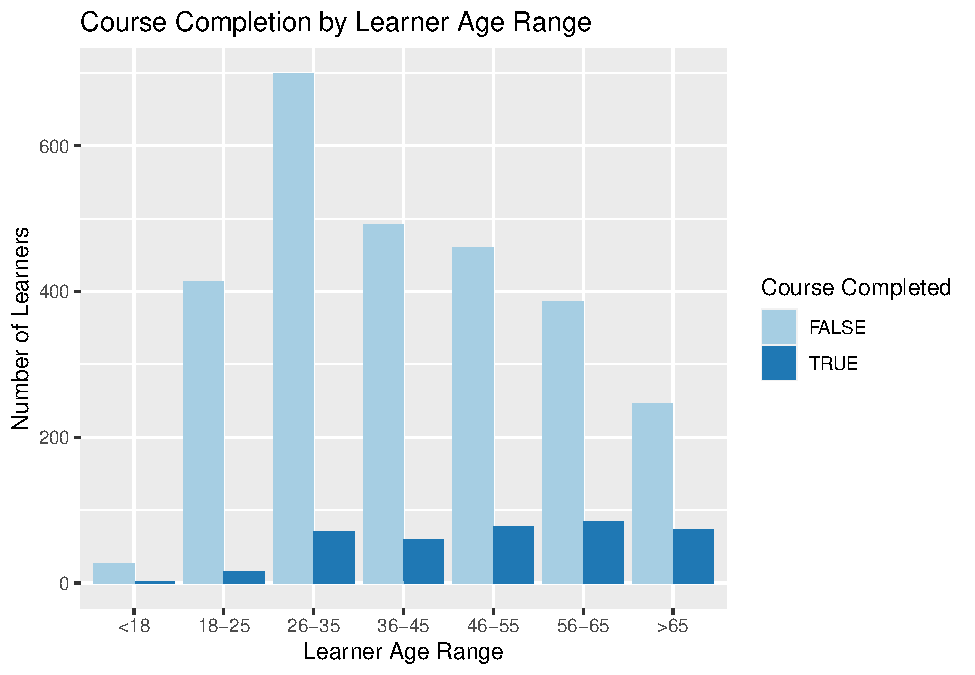
\includegraphics{CSC8631-Report---210431461_files/figure-latex/age_completion-1.pdf}

To better understand the results of this graph, the table below was also
created (the code for calculating the percentages is located in the file
\texttt{eda2.R} which is in the \texttt{src} folder).

\begin{verbatim}
## # A tibble: 8 x 2
##   Success_Rate Percentage
##   <chr>             <dbl>
## 1 Age               12.6 
## 2 <18                4.76
## 3 18-25              4.2 
## 4 26-35              8.8 
## 5 36-45             11.0 
## 6 46-55             14.1 
## 7 56-65             18.0 
## 8 >65               22.9
\end{verbatim}

This table shows us that of learners who declared their age 12.59\%
successfully completed the course. Those who are 65 or older had the
highest chance of success (22.91\%). Learners' chance of success appears
to increase after the age of 26 with learners aged between 18 and 25
having the lowest chance of success (4.20\%).

The graph below was created to better understand the provision of
demographic data by learners who declared their age.

\begin{verbatim}
## Warning: Removed 3 rows containing missing values (geom_bar).
\end{verbatim}

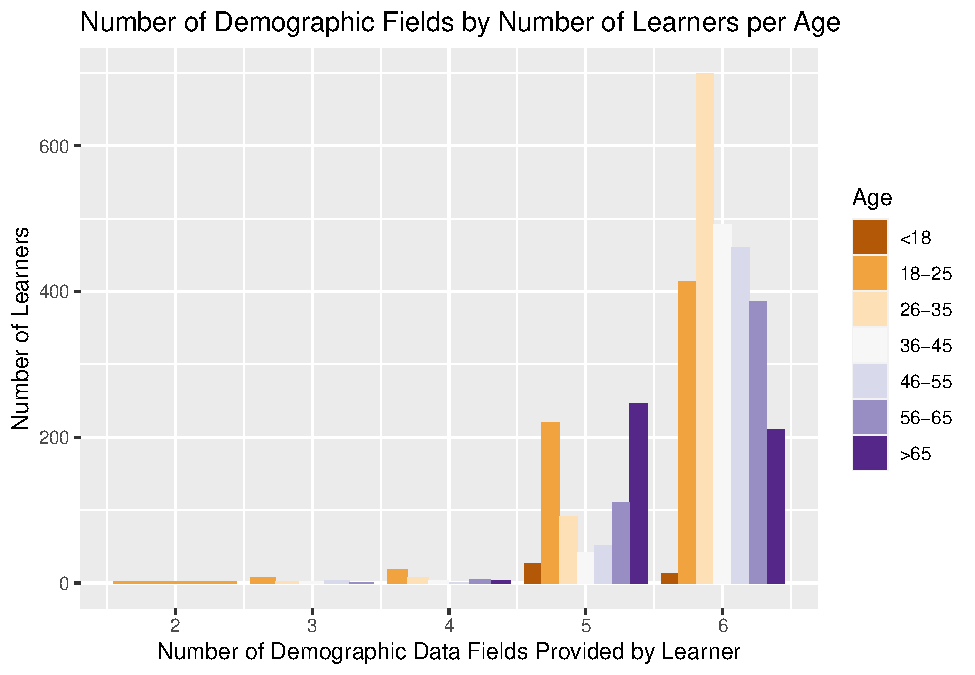
\includegraphics{CSC8631-Report---210431461_files/figure-latex/age_demographics_declared-1.pdf}

This graph indicates that learners in the 26-25 age range are more
likely to share all six demographic data values. Comparatively, if a
learner declares they are over 65, they appear more likely to provide 4
or more demographic data values. This graph also suggests that learners
who share their age range with FutureLearn are also likely to share more
demographic data. To better understand these results, further
exploration is required.

\textbf{Goal 2.3 (Education Level)}

Applying the same analysis process as Goal 2.1 and 2.2, we can determine
that 4135 learners declared their highest education level to
FutureLearn.

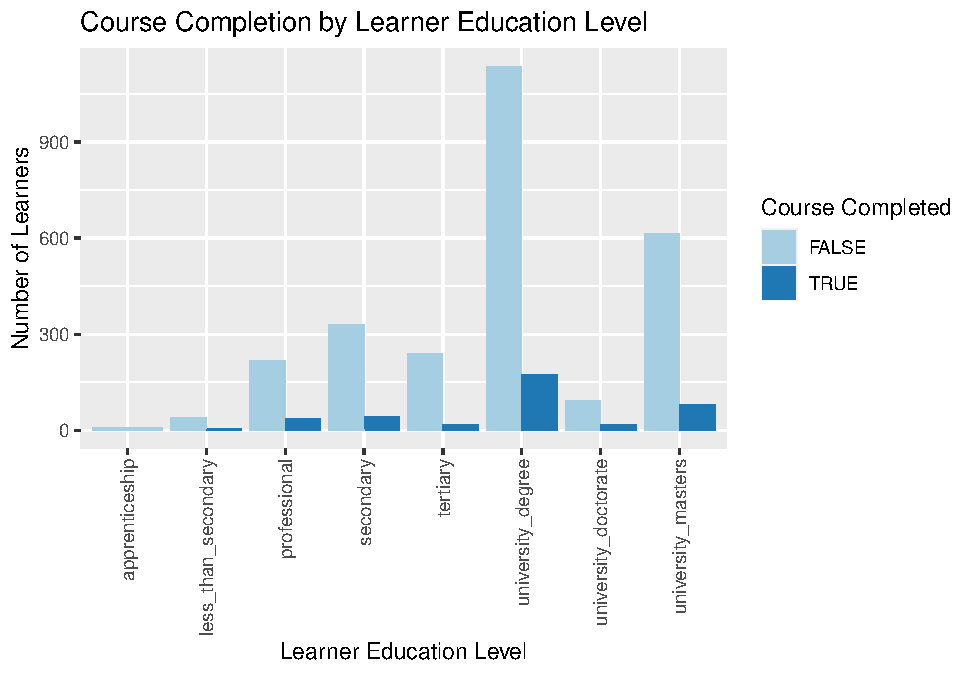
\includegraphics{CSC8631-Report---210431461_files/figure-latex/education_completion-1.pdf}
From this graph, it is unclear which education level correlates to a
higher chance of success for learners. It is clear that there are more
students who enrol in the course who have either a tertiary
qualification of some kind and specifically a university degree or
university masters. To better understand the results of this graph, the
table below was also created (the code for calculating the percentages
is located in the file \texttt{eda2.R} which is in the \texttt{src}
folder).

\begin{verbatim}
## # A tibble: 9 x 2
##   Success_Rate         Percentage
##   <chr>                     <dbl>
## 1 Education                  12.6
## 2 Apprenticeship              0  
## 3 Less_Secondary             10  
## 4 Secondary                  10.9
## 5 Professional               15.0
## 6 Tertiary                   10.5
## 7 University_degree          13.8
## 8 University_masters         11.4
## 9 University_doctorate       15.1
\end{verbatim}

This table shows us that of the learners who declared their highest
education level, 12.55\% successfully completed the course. Those who
held university doctorates (15.07\%) or professional qualifications
(15.04) had the highest chance of success. Those who held
apprenticeships had the lowest chance of success (0\%).

The graph below was created to better understand the provision of
demographic data by learners who declared their highest education level.

\begin{verbatim}
## Warning: Removed 4 rows containing missing values (geom_bar).
\end{verbatim}

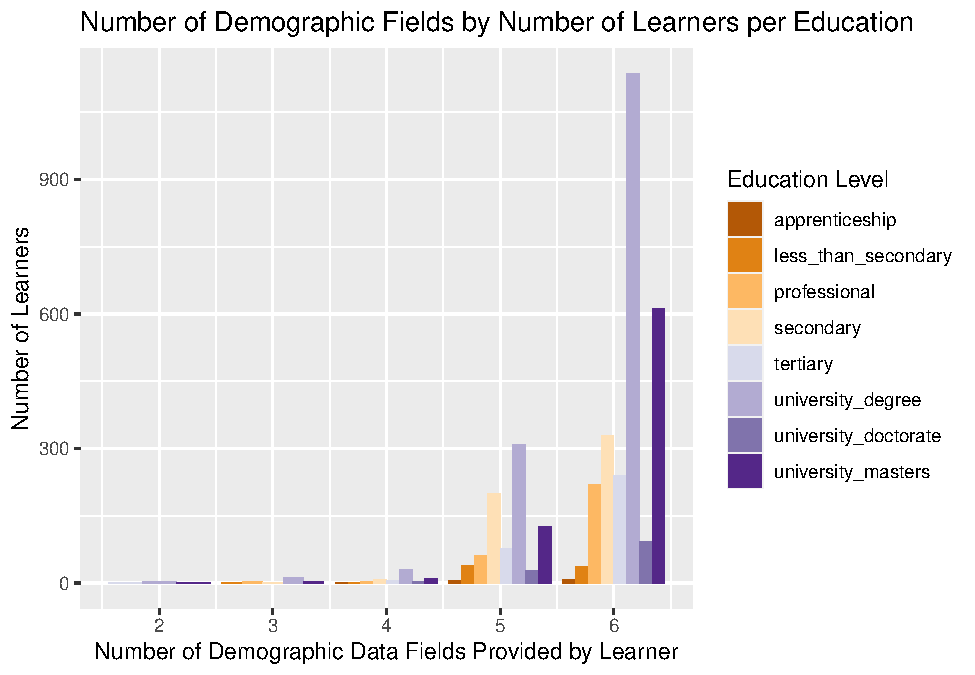
\includegraphics{CSC8631-Report---210431461_files/figure-latex/education_demographics_declared-1.pdf}

This graph suggests that learners with a tertiary qualification of some
kind (tertiary, university\_degree, university\_masters,
university\_doctorate) are more likely to share more demographic data
with FutureLearn. It also indicates that those with apprenticeships and
professional qualifications are less likely to share more demographic
data with FutureLearn. To better understand these results, further
investigation is required.

\textbf{Goal 2.4 (Employment Status)}

Applying the same analysis process as Goal 2.1, 2.2, and 2.3, we can
determine that 4105 learners declared their employment status to
FutureLearn. In the graph below it appears that learners have a higher
chance of success if they are retired.

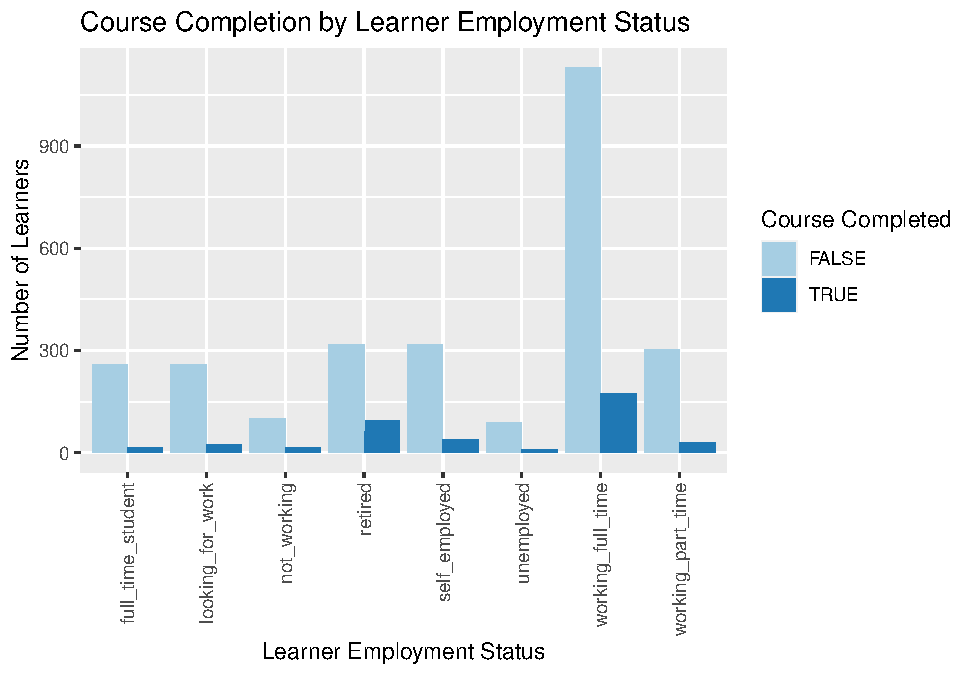
\includegraphics{CSC8631-Report---210431461_files/figure-latex/employment_status_completion-1.pdf}
To better understand the results of this graph, the table below was also
created (the code for calculating the percentages is located in the file
\texttt{eda2.R} which is in the \texttt{src} folder).

\begin{verbatim}
## # A tibble: 9 x 2
##   Success_Rate  Percentage
##   <chr>              <dbl>
## 1 Employment         12.6 
## 2 Student_FT          4.76
## 3 Looking             8.31
## 4 Not_working        11.3 
## 5 Retired            22.4 
## 6 Unemployed          9.36
## 7 Self-employed      10.9 
## 8 Working_FT         13.1 
## 9 Working_PT          9.27
\end{verbatim}

This table shows us that of the 4105 learners who declared their
employment status, 12.57\% completed the course. Learners who are
retired have the highest chance of success (22.45\%) and learners who
are also full time learners have the lowest chance of success (4.76\%).

The graph below was created to better understand the provision of
demographic data by learners who declared their employment status.

\begin{verbatim}
## Warning: Removed 4 rows containing missing values (geom_bar).
\end{verbatim}

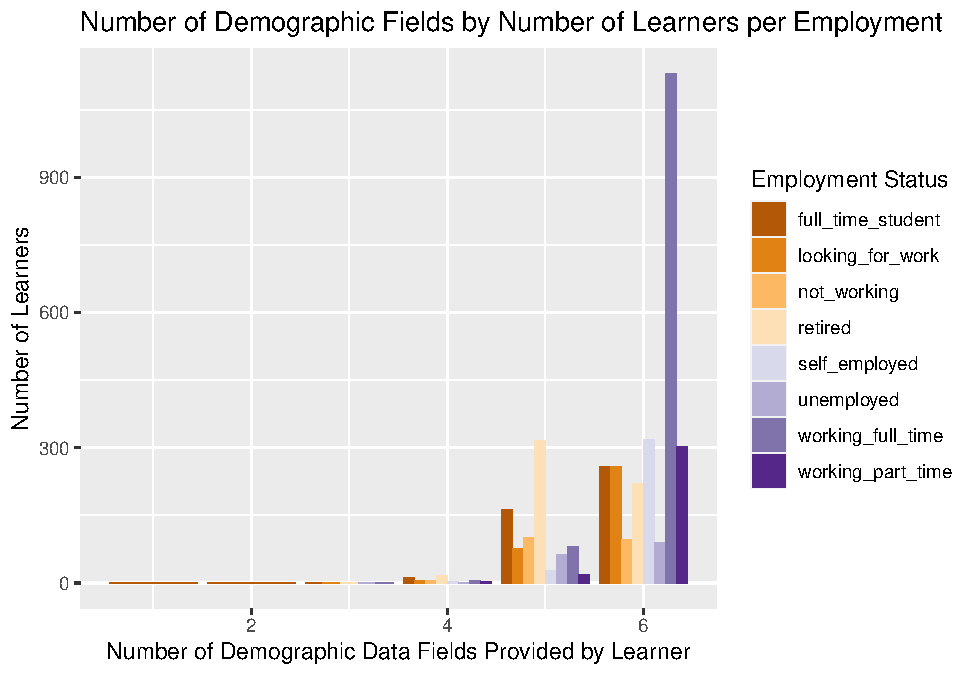
\includegraphics{CSC8631-Report---210431461_files/figure-latex/employment_demographic_declared-1.pdf}
This graph indicates that learners who are working full time may be more
likely to provide FutureLearn with more demographic data (although this
could seem this was as there are more learners who are working full
time). The graph also suggests that those who are retired are more
likely to share five instead of six demographic data values with
FutureLearn, and it would be interesting investigate if these learners
do not share the same demographic data value. To better understand these
results, further exploration is needed.

\hypertarget{data-preparation}{%
\subsection{Data preparation}\label{data-preparation}}

This section outlines the pre-processing steps that produce the data
utilised by this report. The pre-processing code can be found in the
folder called \texttt{munge}. All pre-processing code is included so
that anyone can run the code of this project directly from this report.
The code includes:

\begin{enumerate}
\def\labelenumi{\arabic{enumi}.}
\item
  All seven enrolments data sets are combined into one single data set.
  The enrolments data set is chosen as the majority of demographic data
  provided by learners can be found here.
\item
  This data set is formatted so that all empty cells appear as NA.
\item
  Two filters are created that divide this data by learners who
  completed (complete) and learners who did not complete (incomplete)
  the course.
\item
  A new data set is created for the initial investigation (FL1) so that
  any data transformation or tidying is not applied to the raw data. In
  this new data set, there are seven new columns apply TRUE or FALSE
  based on whether there data in the aforementioned demographic data
  fields and in fully\_participated\_at.
\item
  The learner\_ids for these new columns are identified and are pulled
  together as `ids\_of\_declared\_cols.'
\item
  A new column is created in FL1 that counts the number of TRUEs in the
  aforementioned columns.
\item
  There is also some pre-processing data for the third iteration of
  exploratory data analysis, which is not yet finished and, therefore,
  not included in this report. This code combined the seven archetype
  data sets, joins these to FL1 by learner\_id, and creates a new data
  set of this called FL2. The data needed to assign learners with
  archetypes is potentially demographic data, and so potential insights
  from archetype data sets could offer an interesting comparison to the
  insights from the demographic data in the enrolments spreadsheet.
\end{enumerate}

\hypertarget{evaluation}{%
\subsection{Evaluation}\label{evaluation}}

\hypertarget{assessment-of-data-mining-results-with-respect-to-business-success-criteria}{%
\subsubsection{Assessment of data mining results with respect to
business success
criteria}\label{assessment-of-data-mining-results-with-respect-to-business-success-criteria}}

The process and findings described by this report explore the question:
``Do learners have a higher chance of success the more data they share
with FutureLearn?'' The business success criteria of this project is to
give useful insights into the relationship between learner engagement
and learner success rate. Learners' provision of optional demographic
data is regarded as a proxy for learner engagement. Learner success rate
is regarded as the likelihood a learner completes the course they
enrolled in. Learner engagement and learner success rate are indicators
of learning effectiveness, and the results of the data mining are
interpreted with that context in mind.

\begin{verbatim}
## # A tibble: 15 x 2
##    Success_Rate        Percentage
##    <chr>                    <dbl>
##  1 Gross                     5.78
##  2 No Demographic Data       4.92
##  3 Demographic Data         12.5 
##  4 Gender                   12.3 
##  5 Male                     14.0 
##  6 Other                     7.14
##  7 Age                      12.6 
##  8 >65                      22.9 
##  9 18-25                     4.2 
## 10 Education                12.6 
## 11 Doctorate                15.1 
## 12 Apprenticeship            0   
## 13 Employment Status        12.6 
## 14 Retired                  22.4 
## 15 Student                   4.76
\end{verbatim}

This table shows the overarching success rates as well as the best and
worst success rate for each field of demographic data explored through
this report. The success rate of learners who share demographic data
with FutureLearn is significantly higher (2.55x) than learners who do
not. Interestingly, the success rate for learners who provide
demographic data (12.53\%) is not dissimilar for the overarching success
rate of different demographic fields, such as gender (12.26\%), age
(12.59\%), education (12.55\%), employment status (12.57\%). However,
within these fields of demographic data, the results vary more widely.

The data mining results suggest that FutureLearn is most effective for
people who identify as male (14.02\%), are aged over 65 (22.91\%), hold
a doctorate (15.07\%) or are retired (22.45\%). The results also
indicate that FutureLearn is least effective for people who identify as
other (7.14\%), are between the ages of 18 and 25 (4.20\%), who hold an
apprenticeship (0\%) or are a full time student (4.76\%). The similarity
between some of these data variables suggests that FutureLearn may be
more effective for experienced learners with more time on their hands.
Further investigation is, however, needed to understand whether these
variables refer to particular learner\_ids or pattern for learners.

Initial insights were also collected to better understand the engagement
of those who provided demographic data. The data mining results indicate
that those who share demographic data are likely to provide FutureLearn
with more demographic data. Further investigation is needed to
conclusively determine whether learners have a higher chance of success
the more data they share with FutureLearn; the findings in this report,
however, suggest this holds true.

The findings of the exploratory analysis in this report do produce
useful insights into the relationship between learner engagement and
learner success rate. There is a clear correlation between these
indicators of learning effectiveness, and it does appear that learners
who engage by providing demographic data are more likely to succeed.

\hypertarget{review-of-process}{%
\subsubsection{Review of process}\label{review-of-process}}

This project has been limited by the time available, programming
capabilities, choice of data sets, and scope of the project to focus on
data exploration. The process has been sufficiently effective to
somewhat address the business objective and success criteria. This
project, however, focused more on learners success rate than learner
engagement. If the project should be repeated, further attention should
be given to understanding the impact of the amount of data shared by
students as well as different indicators of learner engagement, such as
archetypes, step activity and leaving survey responses.

\hypertarget{list-of-possible-actions}{%
\subsubsection{List of possible
actions}\label{list-of-possible-actions}}

If the project were to be continued, the possible actions recommended
are:

\begin{enumerate}
\def\labelenumi{\arabic{enumi}.}
\item
  Calculate the success rate for learners of demographic data field that
  also provide one, two, three, four, five and six demographic data
  fields. This will allow us to confirm whether or not there are
  spurious associations.
\item
  Explore the relationship between success rate and other indicators of
  learner engagement (as mentioned above).
\item
  The finding of point 2 could then be compared with the findings for
  demographic data fields outlined by this report. This would help
  FutureLearn and Newcastle University better understand which proxies
  best reflect learner engagement.
\item
  Where groups of learners' success rate are lower, we should explore
  whether or not they responded to the leaving survey and what the most
  common responses are. This will help us to identify how we might
  improve FutureLean's learning effectiveness for them.
\item
  Another interest avenue for exploration is the relationship between
  the learners' success rate and completion time, as this could be
  another indicator of learner engagement.
\end{enumerate}

\newpage

\hypertarget{bibliography}{%
\section*{Bibliography}\label{bibliography}}
\addcontentsline{toc}{section}{Bibliography}

\hypertarget{refs}{}
\begin{CSLReferences}{1}{0}
\leavevmode\vadjust pre{\hypertarget{ref-Learning-Analytics-Conference}{}}%
\emph{1st International Conference on Learning Analytics and Knowledge}.
2011. Banff, Alberta. \url{https://tekri.athabascau.ca/analytics/}.

\leavevmode\vadjust pre{\hypertarget{ref-CRISP-DM}{}}%
Chapman et. al., Juian Clinton, Pete Chapman, and Rudiger Wirth. 2000.
\emph{CRISP-DM 1.0: Step-by-Step Data Mining Guide}.
\url{https://www.the-modeling-agency.com/crisp-dm.pdf}.

\leavevmode\vadjust pre{\hypertarget{ref-FutureLearn}{}}%
FutureLearn. n.d. {``The Power of Social Learning: An Effective Way to
Learn.''}
\url{https://www.futurelearn.com/using-futurelearn/why-it-works}.

\leavevmode\vadjust pre{\hypertarget{ref-EDUCAUSE}{}}%
Long, Phil, and George Siemens. 2011. {``Penetrating the Fog: Analytics
in Learning and Educaton.''} \emph{EDUCAUSE Review} September/October.
\url{https://er.educause.edu/articles/2011/9/penetrating-the-fog-analytics-in-learning-and-education}.

\leavevmode\vadjust pre{\hypertarget{ref-E-learning}{}}%
S. Hubalovsky, M. Hubalovska, and M. Musilek. 2018. {``Assessment of the
Influence of Adaptive e-Learning on Learning Effectiveness of Primary
School Puplis.''} \emph{Computers in Human Behaviour} 92.
\url{https://doi.org/10.1016/j.chb.2018.05.033}.

\leavevmode\vadjust pre{\hypertarget{ref-Bricks}{}}%
Shacklock, Xanthe. 2016. {``From Bricks to Clicks.''} {Policy Connect};
{Higher Education Commission}.

\end{CSLReferences}

\end{document}
